
\documentclass[titlepage]{article}
\setlength{\headheight}{23pt}
\addtolength{\topmargin}{-11pt}

\usepackage{geometry}
\usepackage{tikz}
\usepackage{pgfplots}
\pgfplotsset{compat=1.18}
\pgfplotsset{hide xscale/.style={/pgfplots/xtick scale label code/.code={}}}
\pgfplotsset{hide yscale/.style={/pgfplots/ytick scale label code/.code={}}}
\usepackage{amsmath}
\usepackage{url}
\hyphenation{op-tical net-works semi-conduc-tor}	% Correct bad hyphenation
\usepackage{graphicx}   % For including figures and pictures
\usepackage{float}      % Used to fix location of images i.e.\begin{figure}[H]
\usepackage{fancyhdr}   % For headers and footers
\pagestyle{fancy}
\usepackage{titling}    % To reference title, author, and date
\usepackage{array}      % For fixed-width tables
\usepackage[american]{circuitikz} % Used to draw circuit and block diagrams
\usepackage{appendix}   
\usepackage{colortbl}   % For coloring table cells
\usepackage{enumitem}   % For formatting enumerated lists
\setenumerate[1]{label={(\arabic*)}}
\usepackage[backend=biber,style=numeric,sorting=none]{biblatex}
\addbibresource{references.bib}

% Global CircuiTikZ parameters
\ctikzset{sources/fill=red!20}
\ctikzset{chips/fill=cyan!20}
\ctikzset{electromechanicals/fill=blue!20}
\ctikzset{blocks/fill=green!20}
\ctikzset{amplifiers/fill=yellow!30}
\tikzset{amp/.append style={fill=yellow!30}}
\tikzset{twoport/.append style={fill=cyan!20}}

% The following lines define a new command \nraocite that cites references in NRAO format RD0X by redefining \cite command to remove brackets. \nraoprecite includes a prenote.
\DeclareCiteCommand{\cite}[\mkbibemph{\emph{}}]
  {\usebibmacro{prenote}}
  {\usebibmacro{citeindex}%
   \printtext[bibhyperref]{\usebibmacro{cite}}}
  {\multicitedelim}
  {\usebibmacro{postnote}}
\DeclareCiteCommand*{\cite}[\mkbibemph\emph{}]
  {\usebibmacro{prenote}}
  {\usebibmacro{citeindex}
   \printtext[bibhyperref]{\usebibmacro{citeyear}}}
  {\multicitedelim}
  {\usebibmacro{postnote}}
\newcommand{\nraocite}[1]{[RD0\cite{#1}]}
\newcommand{\nraoprecite}[2][]{[RD0\cite{#2}{, #1}]}

% Suppresses chktex warnings 
% chktex-file 1
% chktex-file 3
% chktex-file 8
% chktex-file 24
% chktex-file 44
% chktex-file 46

% ASSIGN TITLE, AUTHOR, DATE, DOCUMENT NUMBER, STATUS, HERE
\title{Redesign of the Visitor Center Solar Telescope}
\author{Remy Nguyen
    }% <-this % stops a space
\date{June 21, 2023}
\def\docnum{[Assign Here]}
\def\status{\textcolor{red}{Draft}}

% HEADERS AND FOOTERS
% If title is too long, write in text and use \\ to make line breaks
\fancyhead[L]{\textit{\thetitle} \\ \textit{NRAO Doc. \#:} \docnum}
\fancyhead[R]{\textit{\theauthor} \\ \thedate}

 % DOCUMENT STARTS HERE
\begin{document}
%\nobibliography{references.bib}
\definecolor{nraoblue}{rgb}{0.776,0.851,0.945}  % Color of table headers
\setlength{\leftmargin}{1in}
\setlength{\rightmargin}{1in}

\begin{titlepage}
\begin{center}
     
\includegraphics[width=5cm]{images/NRAO Logo Badge.png} \\
     \vspace*{0.5cm}
     \textbf{\Huge\thetitle} \\
     \vspace*{0.5cm}
     \large\docnum \\
     \huge Status: \status \\
     \vspace*{1cm} \large
     % FIRST TABLE HERE
     \begin{tabular}{|m{6.5cm}|m{5cm}|m{2cm}|} \hline
        \rowcolor{nraoblue}
        \textbf{Prepared By} & \textbf{Organization} & \textbf{Date} \\ \hline
        R. Nguyen & NRAO Electronics Div. & 6/21/2023 \\ 
        \hline
    \end{tabular} \\
    \vspace*{1cm}
    \begin{tabular}{|m{3cm}|m{3.5cm}|m{7cm}|} \hline
        \rowcolor{nraoblue}
        \textbf{Approvals} & \textbf{Organization} & \textbf{Signatures} \\ \hline
    \end{tabular}
    \renewcommand{\arraystretch}{1.5}
    % CONTENT OF SECOND TABLE HERE
    \begin{tabular}{|m{3cm}|m{3.5cm}|m{7cm}|}
        T. Mobraten & NRAO Electronics Division &  \\ 
        \hline
        S. Wimbrow & NRAO Electronics Division &  \\ 
        \hline
        D. Schafer & NRAO Electronics Division &  \\ 
        \hline
    \end{tabular} \\
    \renewcommand{\arraystretch}{1}
    \vspace*{1cm}
    \begin{tabular}{|m{3cm}|m{3.5cm}|m{7cm}|} \hline
        \rowcolor{nraoblue}
        \textbf{Released By} & \textbf{Organization} & \textbf{Signature} \\ \hline
    \end{tabular}
    \renewcommand{\arraystretch}{2}
    % CONTENT OF THIRD TABLE HERE
    \begin{tabular}{|m{3cm}|m{3.5cm}|m{7cm}|}
        D. Schafer & NRAO Electronics Division &  \\ 
        \hline
    \end{tabular}
    \renewcommand{\arraystretch}{1}
\end{center}
\end{titlepage}


\tableofcontents
\listoffigures
\thispagestyle{fancy}
\newpage

\section{Introduction}

\subsection{Purpose}
Located behind the Visitor Center at the Very Large Array (VLA) is a radio telescope that converts RF solar energy into a DC voltage through amplification. It was originally constructed in 2013 and is no longer functioning as of June 2023. Weathered components and lack of sufficient documentation to repair the telescope to its original state has warranted a redesign of the entire system to be more appealing to visitors and resistant to wear.

\subsection{Scope}
This document will describe the design choices made in development of the new solar telescope. Calculations and experiments to support design decisions will be demonstrated along with constraints and requirements.


\section{Related Documents and Drawings}
\subsection{Applicable Documents}
The following documents may not be directly referenced herein, but may provide necessary context or supporting material.
\begin{center}
\begin{tabular}{|m{2cm}|m{7cm}|m{2.5cm}|} \hline
    \rowcolor{nraoblue}
    Ref. No. & Document Title & Rev/Doc. No.\\ \hline
    AD01 & Desiderata for Solar Observing with the EVLA & EVLAM\_70 \\ 
    \hline
    AD02 & EVLA Hardware Modifications in Support of Solar Observing & EVLAM\_72 \\
    \hline
\end{tabular}
\end{center}

\subsection{Reference Documents}
The following documents are referenced within this text:
\begin{center}
\renewcommand{\arraystretch}{1.2}
\begin{tabular}{|m{2cm}|m{7cm}|m{2.5cm}|} \hline
    \rowcolor{nraoblue}
    Ref. No. & Document Title & Rev/Doc. No.\\ \hline
    RD01 & \citefield{solartemp}{title} & 0001 \\ \hline
    RD02 & \citefield{aeh}{title} & 0002 \\\hline
    RD03 & \citefield{tora}{title} & 0003 \\\hline
    RD04 & \citefield{xbandvla}{title} & 0004 \\\hline
    RD05 & \citefield{sfd1986}{title} & 0005 \\\hline
\end{tabular}
\renewcommand{\arraystretch}{1}
\end{center}

\section{System Overview}
The heart of the telescope is an conical corrugated X-band horn antenna originally used to receive Voyager transmissions at 8.4 GHz; this is to be unchanged in the redesign. Power is supplied through a 15 volt linear DC power supply located inside the visitor center in order to eliminate radio frequency interference (RFI) caused by AC power and switching power supplies.

As the telescope is pointed towards the sun, RF energy is received by the antenna and amplified. A rectifying circuit converts the RF power into a DC voltage and further amplifies it before outputting to a voltmeter. The DC gain should be adjusted so that as the telescope is pointed towards the sun with clear skies, the voltmeter should read a maximum 5 volts; as the telescope is pointed towards the ground or away from the sun, the voltmeter reading should decrease noticeably.

\subsection{Requirements}
Being a visitor center attraction, the device must be engaging and appealing to visitors. In order to achieve this, the device must be at least partially transparent to show visible electronics and have a voltmeter that is driven by solar energy. The enclosure of the previous design was made of some sort of polycarbonate material which suffered from yellowing in the sun. Additionally, small computer fans with a mesh screen mounted directly to the enclosure were used to decrease operating temperature but allowed dust to accumulate over the years. In essence, the new design goals are as follows:
\begin{enumerate}
    \item Utilizes a transparent enclosure or panel to view electronics, ideally one which will not yellow or fade easily.
    \item Must be dustproof and resilient to accumulation of debris inside the enclosure while still venting heat from electronics.
    \item Use readily available parts when possible to keep costs low.
    \item Electronics must be powered by a fixed DC linear power supply and be easily serviceable.
\end{enumerate}

\subsection{Architecture}
\begin{figure}[!ht]
    \begin{center}
        \begin{circuitikz}
            \draw(0, 0)
            node[
                rxantenna, 
                xscale=-1,
                label = {[xshift=-1.4cm, yshift=-0.5cm]X-band feed}
                ]{}
            to[amp = RF Gain Block, boxed] ++ (2, 0)
            to[bandpass = Filter] ++ (2,0)
            to[detector = Rectifier] ++ (2,0)
            to[amp = DC Gain Block, boxed] ++ (3,0)
            to[qvprobe = Voltmeter] ++ (2,0)
            -| ++ (0.5,-1) node[ground]{};
        \end{circuitikz}
    \caption{RF signal block diagram}\label{fig:rfblock}
    \end{center}
\end{figure}
Many of the RF components were either reused from the previous design or gathered at no cost. The RF gain block shown in Fig.~\ref{fig:rfblock} and \ref{fig:rfgain} utilizes 4 low noise amplifiers (LNAs) and an attenuator to provide better impedance matching. The first 3 LNAs are Mini-Circuits ZX60-83LN-S+ which provide a measured 15dB of gain at 8.4 GHz each; they are followed by a single 6 dB attenuator and an ALS-04-0149 LNA in that order. The ALS-04-0149 does not have a readily available datasheet but measured 27dB of gain at 8.4 GHz.
\begin{figure}[!ht]
    \begin{center}
        \begin{circuitikz}
            \draw(0, 0)
            to[short, o-] ++ (0.5,0)
            to[amp] ++ (2, 0)
            to[amp, l=ZX60-83LN-S+ (x3)] ++ (2, 0)
            to[amp] ++ (2, 0)
            to[twoport, name=tp, fill=green!20] ++ (2, 0)
            to[amp = ALS-04-0149] ++ (2, 0)
            to[short, -o] ++ (0.5,0);
            \draw (tp.center)
            node[resistorshape, anchor = center, rotate = 90, scale = 0.8]{};
            \draw (tp.north)
            node[anchor = south]{-6 dB};
        \end{circuitikz}
    \caption{RF gain block}\label{fig:rfgain}
    \end{center}
\end{figure}

The bandpass filter does not have an attached datasheet but it resembles an equiripple filter and measured a 3 dB passband of about 7.8--8.9 GHz.

The rectifier and DC gain block are integrated into a PCB with SMA connectors. The former utilizes an Analog Devices ADL5902, providing a linear-in-decibel output that can be scaled by the choice of resistors on the board or the following gain element. The DC gain block utilizes an LM358 op amp with an adjustable gain via potentiometer.

    

\subsection{Power Distribution}
As part of the effort to make the telescope more modern and visually appealing, the protoboard on the previous design was replaced with a dual layer PCB which contains the voltage regulators, the RF power detector IC, and the dual noninverting op amps. 15 volts is used to bias the ALS-04-0149 LNA and op amps, whereas 5 volts is used to power the ADL5902, the ZX60-83LN-S+ LNAs, and the fans.
\begin{figure}[!ht]
\begin{center}
\ctikzloadstyle{legacy}
\ctikzset{bipoles/twoport/width=1}
\begin{circuitikz}
    \draw(0,0)
    to[vsource, v_ = $V_{in}$] ++ (0,-3)
    node[tlground]{}
    (0, 0) -- ++ (1,0)
    % U1
    to[twoport, t=L7815, name=u1, l=U1] ++ (1.5,0)
    -- ++ (1,0) node[anchor=south, name=15v]{15 V}
    -- ++ (1,0)
    % U2
    to[twoport, t=L7805, name=u2, l=U2] ++ (1.5,0)
    -- ++ (1,0) node[anchor=south, name=5v1]{}
    -- ++ (2,0) node[anchor=south, name=5v2]{5 V}
    -- ++ (2,0) node[anchor=south, name=5v3]{}
    to[short, -o] ++ (1,0);
    % Amplifiers
    \draw(15v.south)
    to[short, f = 150 mA] ++ (0,-2)
    node[plain mono amp, anchor=up, scale = 0.75, name = lna1]{LNA};
    \draw(5v1.south)
    to[short, f = 75 mA] ++ (0,-2)
    node[plain mono amp, anchor=up, scale = 0.75, name = lna2]{LNA};
    \draw(5v2.south)
    to[short, f = 75 mA] ++ (0,-2)
    node[plain mono amp, anchor=up, scale = 0.75, name = lna3]{LNA};
    \draw(5v3.south)
    to[short, f = 75 mA] ++ (0,-2)
    node[plain mono amp, anchor=up, scale = 0.75, name = lna4]{LNA};
    \draw(lna1.out) to[open, o-o] (lna2.in);
    \draw(lna2.out) -- (lna3.in);
    \draw(lna3.out) -- (lna4.in);
    \draw(lna1.in) to[short, o-] ++ (0,0);
    \draw(lna4.out) to[short, o-] ++ (0,0);
    % ADL5902
    \draw(5v1.south)
    to[short, f_ = 90 mA] ++ (0,2)
    node[qfpchip, anchor = pin 3, hide numbers, external pins width = 0, label = {[scale = 0.8]ADL5902}, name = U3]{}
    (U3.north) node[anchor = south]{U3};
    % Fan
    \draw(5v3.south)
    to[short, f_ = 40 mA] ++ (0,2)
    node[elmech, anchor = bottom, name = fan]{M}
    (fan.top) node[anchor = south]{Fan};
\end{circuitikz}
\caption{DC power distribution block diagram}\label{fig:dcblock}
\end{center}
\end{figure}


\section{Design Calculations}
The rectifier block has a linear region of RF input power to output voltage; the purpose of the gain elements is to shift the signal power into this linear region of operation. At the frequency and temperature of operation, the linear region was chosen to be -30 dBm to 0 dBm based on information available in the datasheet. The next section will show the calculations performed in order to determine how much gain is necessary to reach the linear region of the rectifier.


\subsection{Calculating Antenna Input Power}
In order to determine how much gain to implement, the antenna input power and range of the linear region must be known. The linear region is fixed with a 30 dB dynamic range but antenna input power may vary daily and annually depending on solar cycle\nraoprecite[Fig.~2]{solartemp}.

The first step will be to determine the range of antenna input power when pointed at the sun. Instantaneous power received by the antenna from a celestial source in watts, $P_R$, is defined by Eq.~\ref{eq:power}
\begin{equation}
    P_R = S A_e \Delta f
\label{eq:power}
\end{equation}
where $S$ is the source flux density in W m$^{-2}$ Hz$^{-1}$, $A_e$ is the effective aperture area in m$^2$, and $\Delta f$ is the receiver bandwidth in Hz\nraoprecite[eq.~(41-2)]{aeh}. Effective aperture can be calculated using measurements of the antenna as shown in Eq.~\ref{eq:ae}
\begin{equation} \label{eq:ae}
\begin{split}
    A_e &= \frac{\lambda^2}{4\pi}G \\
    &= \frac{\pi d^2}{4} \eta_a
\end{split}
\end{equation}
where $G$ is linear antenna gain, $d$ is the diameter of the circular horn at the aperture, and $\eta_a$ is the unitless aperture efficiency\nraoprecite[pg.~(15-27)]{aeh}\nraoprecite[eq.~(5.58)]{tora}. An ideal horn antenna has an $\eta_a$ of 0.522. The calculations for this design will use an approximate value of 0.5\footnote{The x-band horn measured an estimated aperture efficiency of 0.62$\pm$0.03 but only when mounted to the VLA dish\nraocite{xbandvla}. This design will assume the antenna to be a standard horn antenna.}. The antenna diameter at the opening measured to be 34 cm, resulting in an effective area of 0.0454 m$^2$ or -13.4 dB m$^2$.

Receiver bandwidth $\Delta f$ can be defined by the bandwidth of the bandpass filter in Fig.~\ref{fig:rfblock}, thus, the received power $P_R$ is more representative of channel power without any amplification, rather than antenna output power, as the antenna is a wideband feed with a higher bandwidth than the filter. In this case, receiver bandwidth is defined to be 1100 MHz or 90.4 dB Hz.

Lastly, values for solar flux density $S$ must be found within the operating frequency. Ho \textit{et al.}\nraocite{solartemp} measured mean, minimum, and maximum values for solar flux density at 2800 MHz and 8800 MHz but only numbers for the former are shown in the text. However, they claim that solar flux density at 8800 MHz are higher by a factor of 2.17 on average, thus, the mean, minimum, and maximum values at 2800 MHz can be multiplied by 2.17 to achieve approximate values for $S$. Additionally, solar brightness temperature shown in~\nraoprecite[Fig.~5]{solartemp} can be used to calculate solar flux density via~\nraoprecite[eq.~(2)]{solartemp}. The former method shows higher dynamic range and is shown in Table~\ref{tab:sfd} in solar flux units\footnote{One solar flux unit (SFU) is equal to $10^{-22}$ W m$^{-2}$ Hz$^{-1}$.}.
\begin{table}[!ht]
\centering
\begin{tabular}{c|c|c|c}
    & $S_{\min}$ & $S_{\mu}$ & $S_{\max}$ \\ \hline
    2.8 GHz & 70 SFU & 150 SFU & 280 SFU \\
    8.8 GHz & 152 SFU & 326 SFU & 608 SFU
\end{tabular}
\label{tab:sfd}
\caption{Solar Flux Density $S$ at 8.8 GHz extrapolated by multiplying $S$ in~\nraocite{solartemp} at 2.8 GHz by a factor of 2.17.}
\end{table}

With values for $S$, $A_e$, and $\Delta f$ found, we can now calculate the antenna channel power $P_R$ with equation~\ref{eq:power} to be -87.9 dBm at $S_{\mu}$. Calculating $P_R$ at $S_{\min}$ and $S_{\max}$ show a roughly $\pm$3 dBm variation in $P_R$. Note that this calculation assumes that solar flux density is constant across the entire frequency range of the receiver. This is a limitation of available information on solar flux density; in practice, $S$ generally increases with frequency\nraocite{sfd1986}.


\subsubsection{Antenna Power Measurements}
In order to confirm these calculations, the antenna was connected to an Anritsu Model MS2720T/720 Spectrum Analyzer centered at 8.4 GHz spanning 100 MHz and pointed towards the sun.
\begin{figure}[H]%[!ht]
\begin {center}
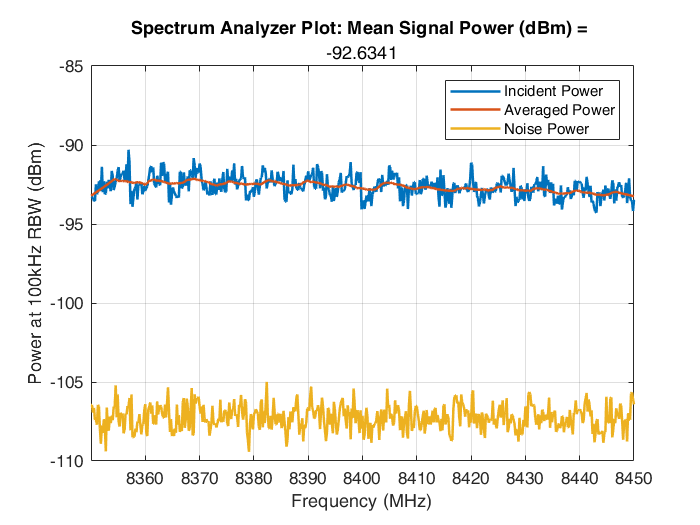
\includegraphics[width=0.65\textwidth]{images/specan1.png}
\caption{Signal trace with 30 dB of gain from two ZX60-83LN-S+ LNAs. Resolution bandwidth is 100 kHz.}
\label{fig:specan1}
\end {center}
\end{figure}
The Anritsu is not capable of performing channel power measurements, so, assuming the mean signal power in Fig.~\ref{fig:specan1} can be extrapolated to the entire receiver bandwidth, channel power is calculated as follows:
\begin{align*}
    P_R &= P_{\mu} - G_{dB} - \left(RBW\right)_{dB} + \left(BW\right)_{dB}\\
        &= -92.6\ \text{dBm} - 30 - 50 + 90.4\\
        &= -82.2\ \text{dBm}
\end{align*}
This measurement is about 5 dB greater than calculated but is within the degree of accuracy necessary for this design. It's possible this error was caused by assuming equal power throughout the entire passband, or due to the fact that this operating frequency is outside the bandwidth of the amplifiers used, thus resulting in nonlinear gain across frequency.

The 4 LNAs and single 6dB attenuator chosen provide a combined 66 dB of gain; thus, the ADL5902 incident power would measure approximately -16 dBm when pointed at the sun, well within its linear operating region.


\appendix
\section{Appendix Title}


\end{document}


